% @Author: AnthonyKenny98
% @Date:   2020-02-29 14:51:44
% @Last Modified by:   AnthonyKenny98
% @Last Modified time: 2020-03-01 08:07:28
\begin{figure}[H]
\begin{center}

    % Subfigure A
    \begin{subfigure}{\textwidth}
    \begin{center}
    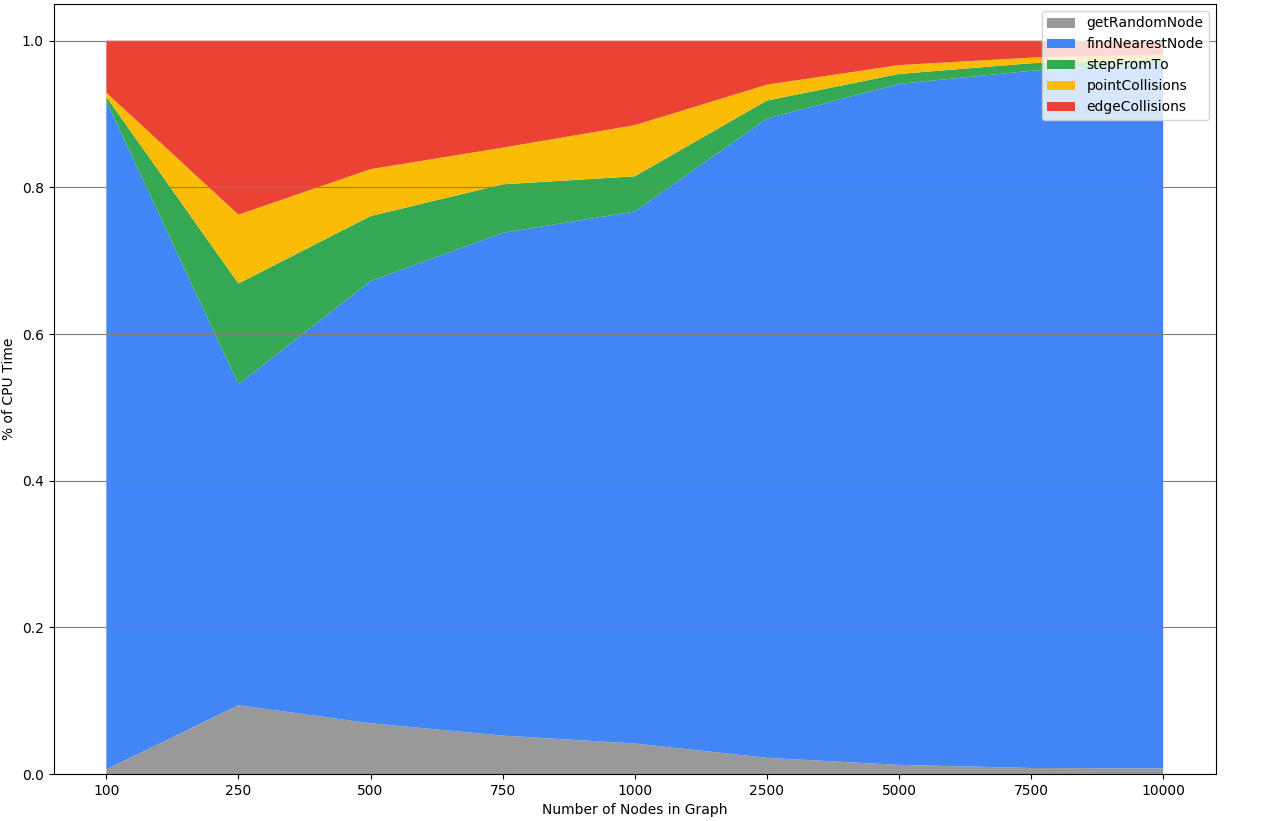
\includegraphics[width=\linewidth,height=0.3\paperheight]{chapters/chapter2/img/profiling/4x4x4/performance.png}
    \caption{4x4x4 Configuration Space}
    \label{subfig:4x4x4rrt}
    \end{center}
    \end{subfigure}
    % 
    % Subfigure B
    \begin{subfigure}{\textwidth}
    \begin{center}
    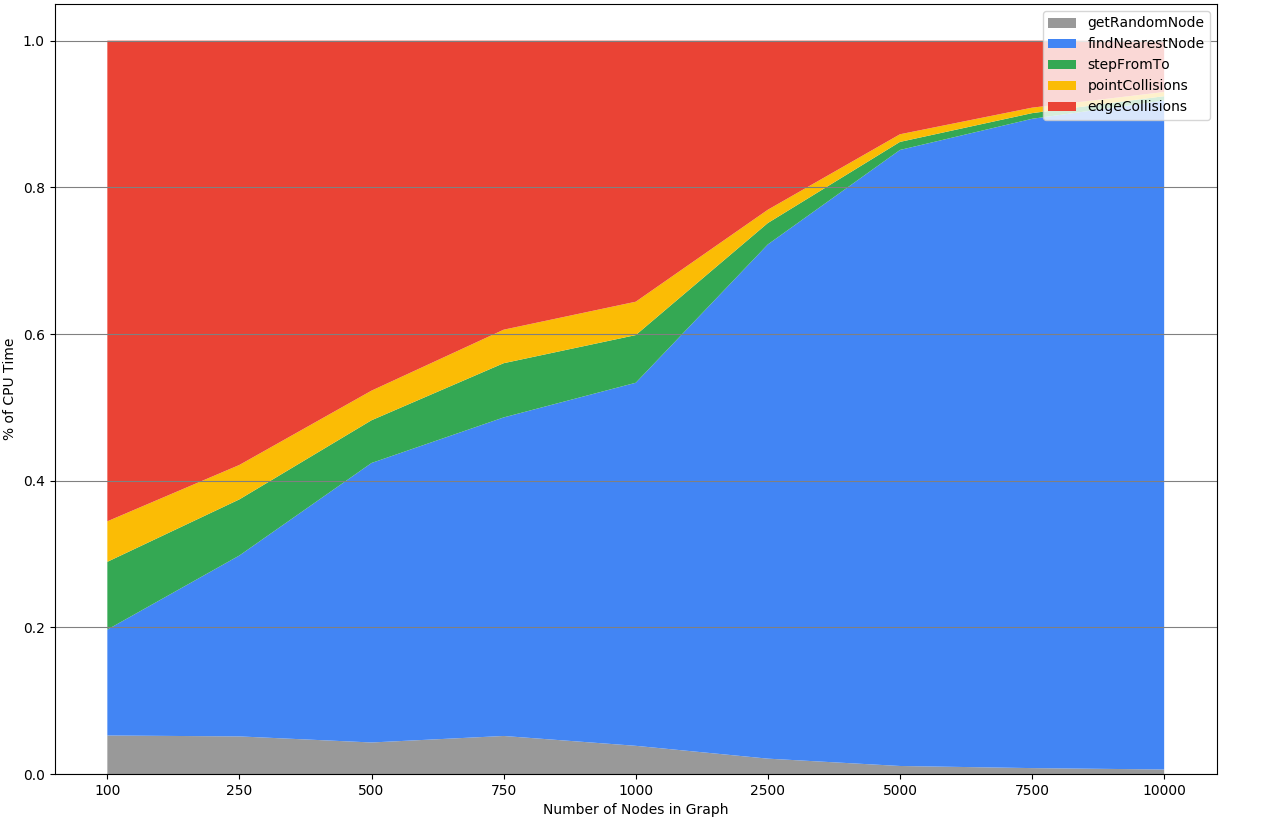
\includegraphics[width=\linewidth,height=0.3\paperheight]{chapters/chapter2/img/profiling/8x8x8/performance.png}
    \caption{8x8x8 Configuration Space}
    \label{subfig:8x8x8rrt}
    \end{center}
    \end{subfigure}
    % Caption and Label
    \caption{\ac{RRT} Functions as a \% of Total CPU Exectution Time}
\end{center}
\end{figure}

\newpage
\begin{figure}[H]\ContinuedFloat
\begin{center}
    % 
    % Subfigure C
    \begin{subfigure}{\textwidth}
    \begin{center}
    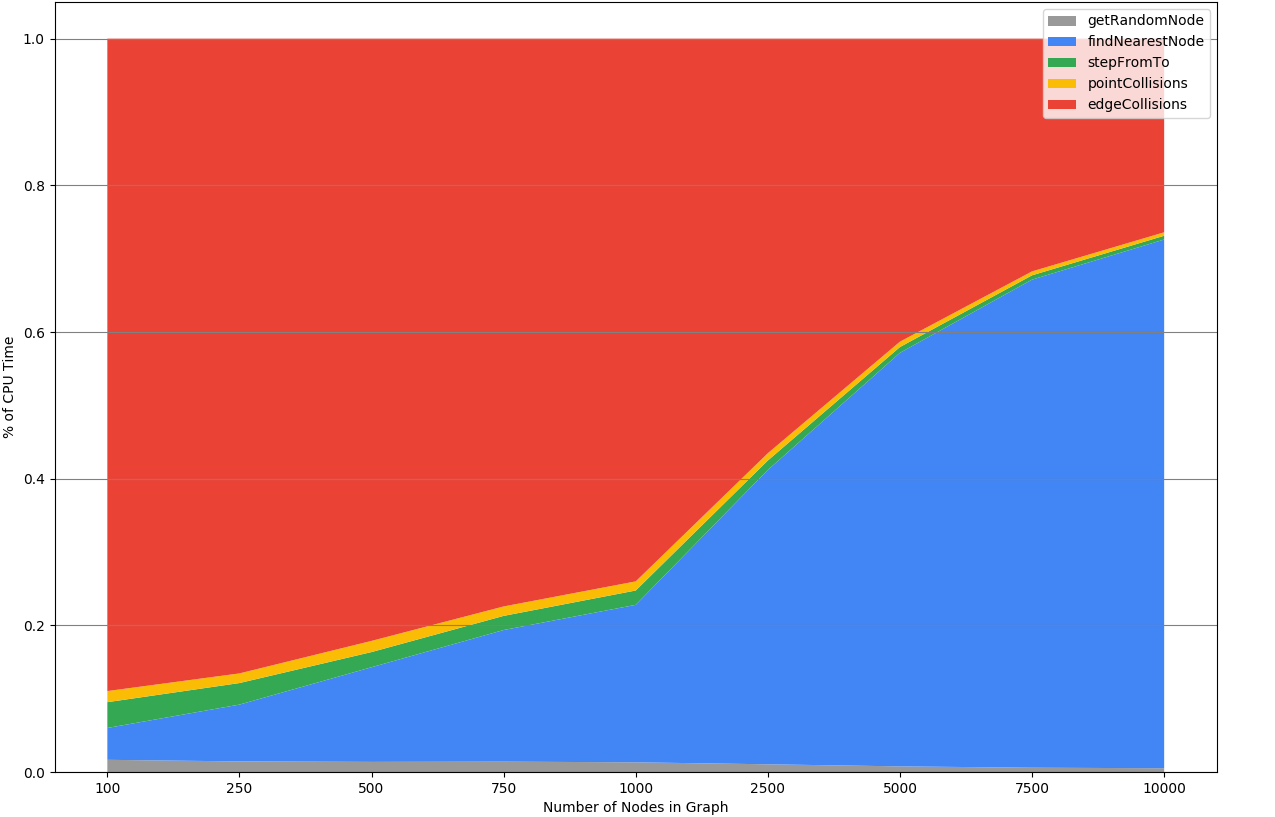
\includegraphics[width=\linewidth,height=0.3\paperheight]{chapters/chapter2/img/profiling/16x16x16/performance.png}
    \caption{16x16x16 Configuration Space}
    \label{subfig:16x16x16rrt}
    \end{center}
    \end{subfigure}
    % 
    % Subfigure D
    \begin{subfigure}{\textwidth}
    \begin{center}
    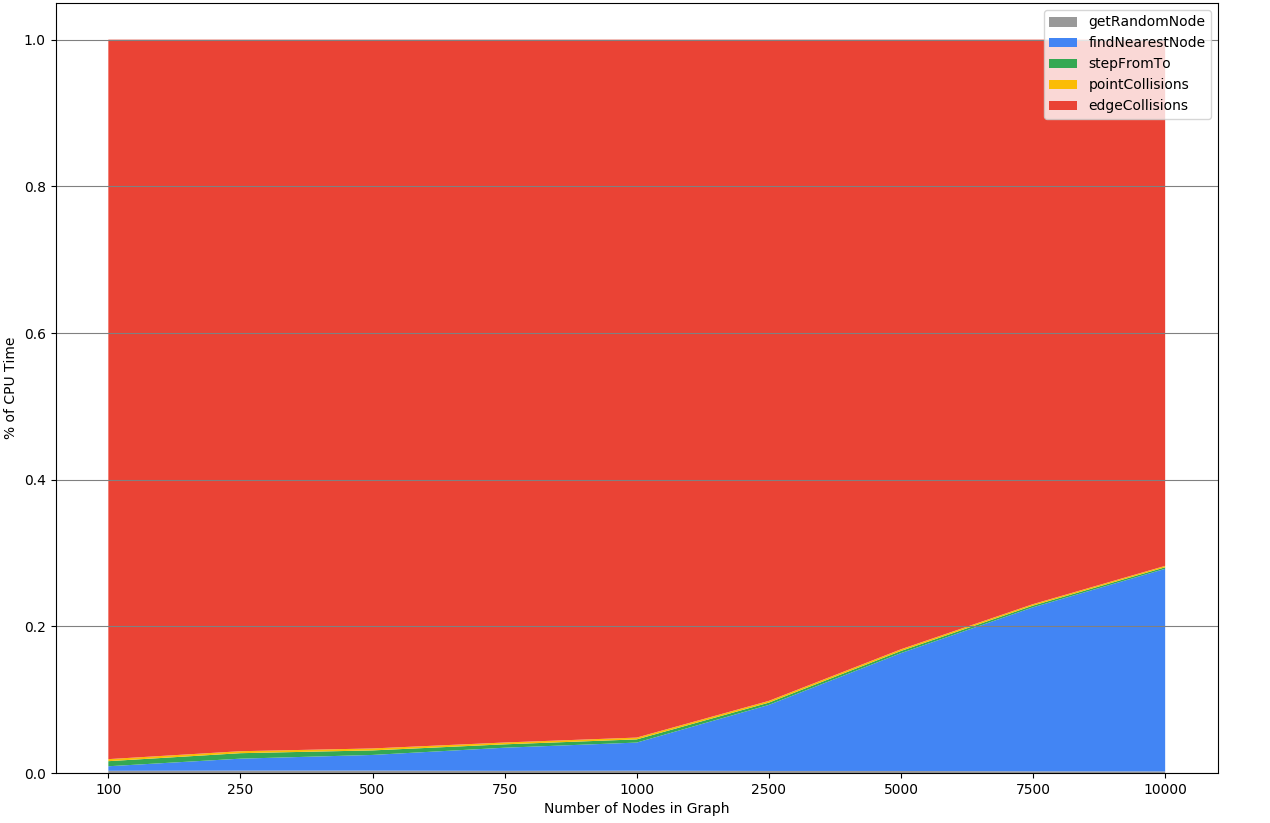
\includegraphics[width=\linewidth,height=0.3\paperheight]{chapters/chapter2/img/profiling/32x32x32/performance.png}
    \caption{32x32x32 Configuration Space}
    \label{subfig:32x32x32rrt}
    \end{center}
    \end{subfigure} 
    
    % Caption and Label
    \caption{\ac{RRT} Functions as a \% of Total CPU Exectution Time (cont.)}
    \label{fig:rrt_profiling}
\end{center}
\end{figure}
\todo[inline]{Change Y axis to \% and increase text size}